\documentclass[11pt,a4paper]{article}
\usepackage[utf8]{inputenc}
\usepackage[spanish]{babel}
\usepackage{amsmath}
\usepackage{amsfonts}
\usepackage{amssymb}
\usepackage{graphicx}
\usepackage{geometry}
\usepackage{fancyhdr}
\usepackage{enumitem}

% Configuración de márgenes
\geometry{left=2cm,right=2cm,top=2.5cm,bottom=2.5cm}

% Encabezado y pie de página
\pagestyle{fancy}
\fancyhf{}
\lhead{Asistente de IA - Física}
\rhead{Cinemática: MRU y MRUA}
\cfoot{Página \thepage}

\begin{document}

\begin{center}
    \LARGE \textbf{Guía de Ejercicios: Cinemática} \\
    \vspace{0.2cm}
    \large Resolución de Problemas y Análisis Gráfico
\end{center}

\vspace{0.5cm}

\section*{Instrucciones}
Lea atentamente cada enunciado y observe el gráfico adjunto. Resuelva utilizando las ecuaciones de movimiento correspondientes y verifique su resultado con la sección de respuestas al final.

\vspace{0.5cm}

% --- BLOQUE DE EJERCICIOS ---
% Este marcador será reemplazado por el script de Python
\subsection*{Ejercicio 1}
Un ciclista mantiene un ritmo constante de 7.0 m/s durante 22.0 segundos. Si comenzó en el origen de coordenadas (0 m), ¿en qué punto se encuentra ahora?

\begin{center}
    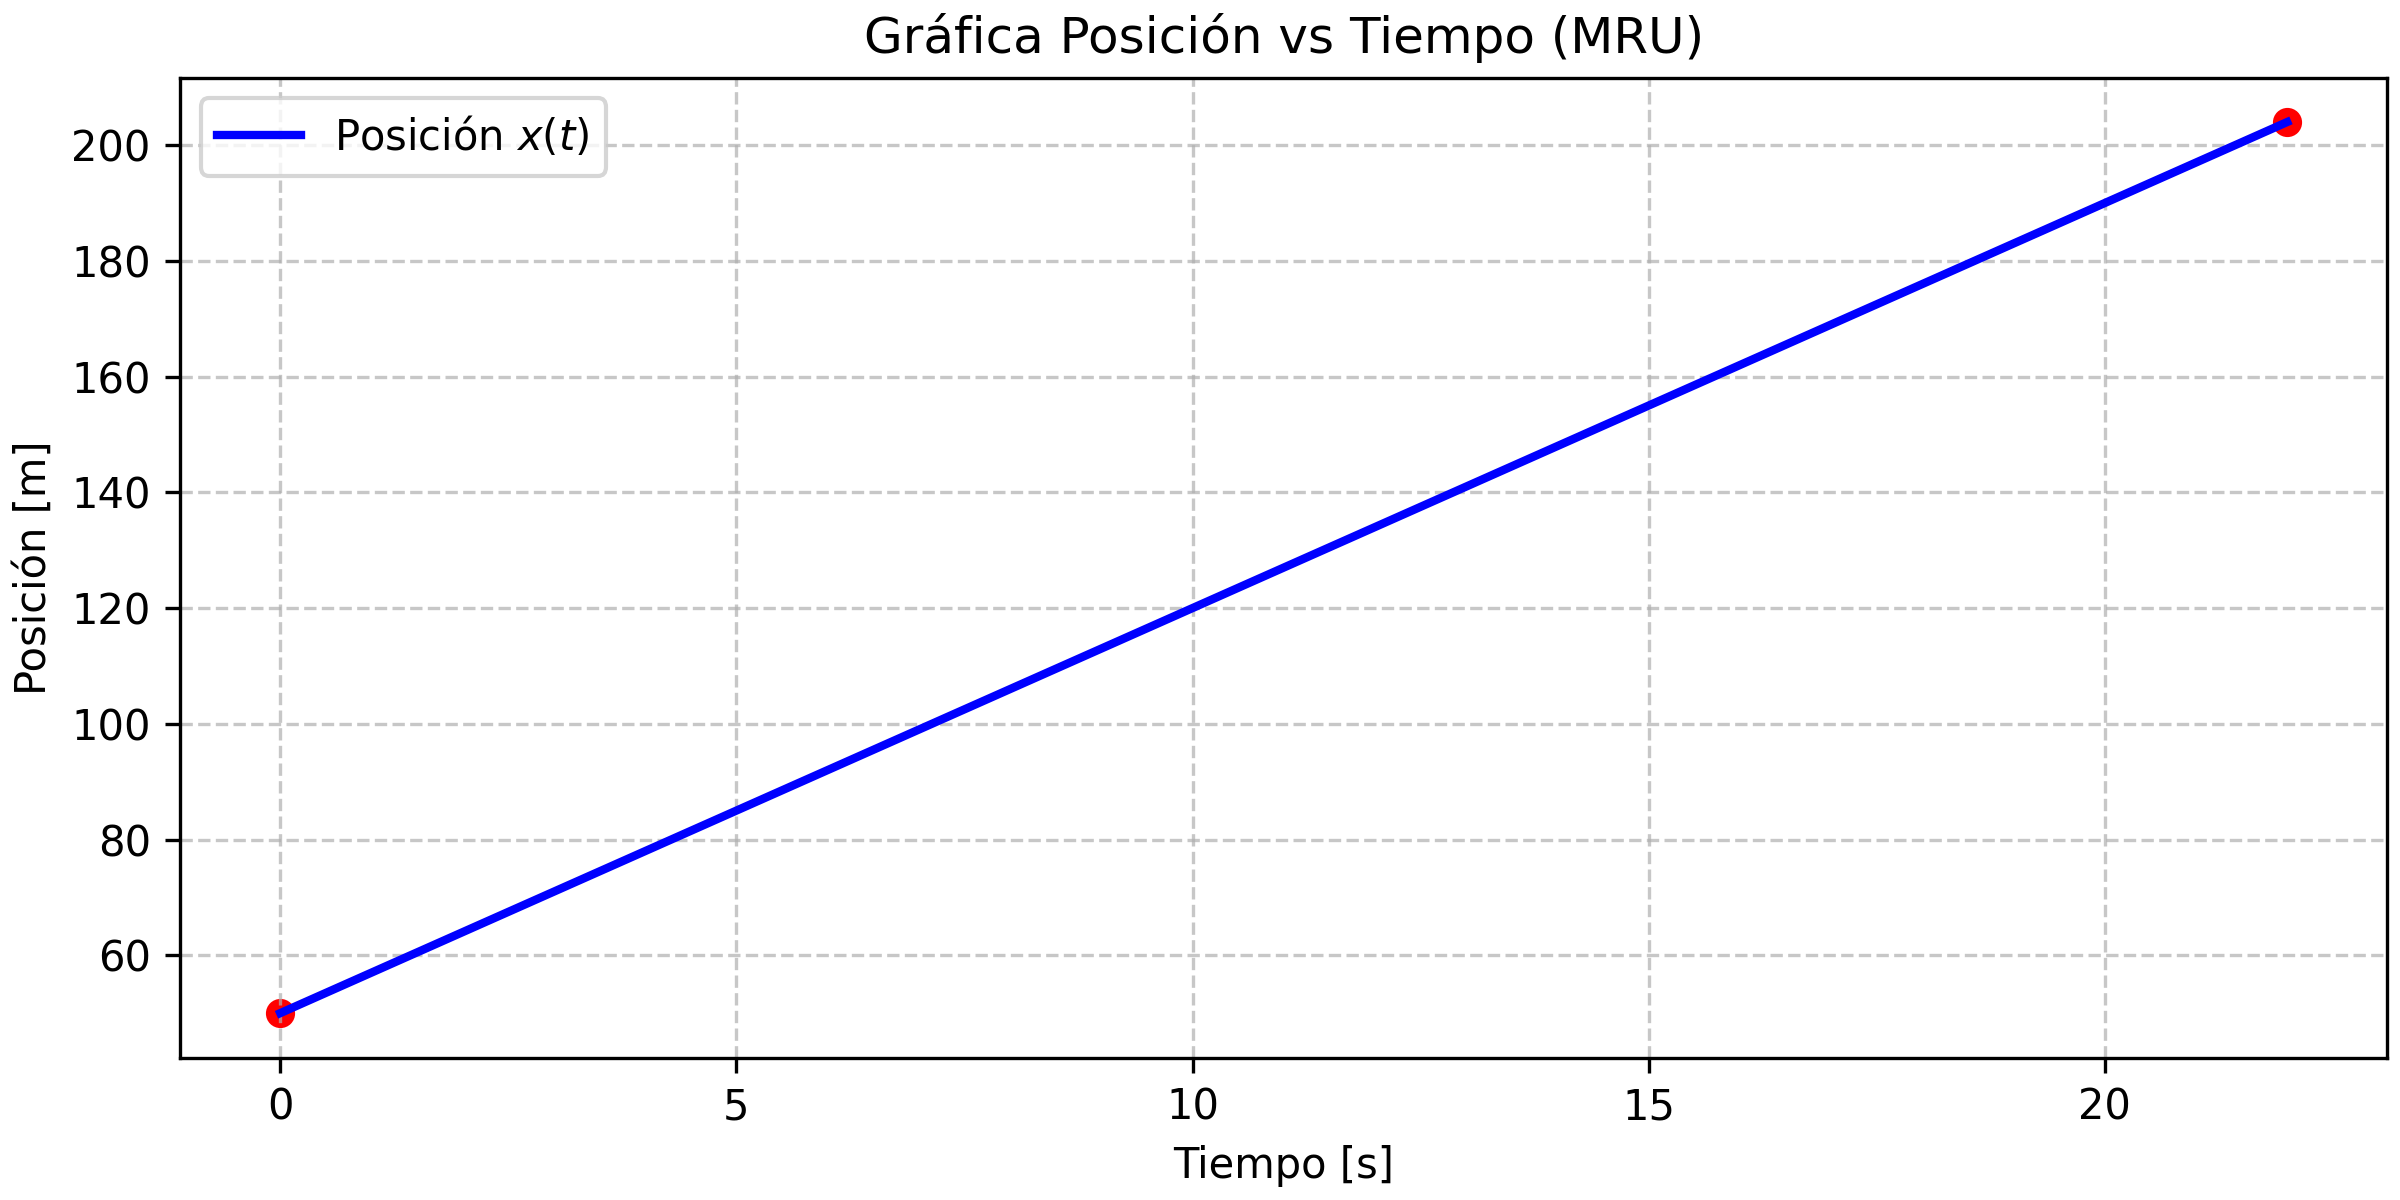
\includegraphics[width=0.8\textwidth]{grafico_1.png}
\end{center}

\vspace{0.5cm}
\textbf{Espacio para Resolución:}
\hrulefill
\vspace{1.5cm}
\hrulefill
\vspace{1.5cm}
\hrulefill
\vspace{1cm}

\subsection*{Ejercicio 2}
Un proyectil es disparado con una velocidad inicial de 2.0 m/s y una aceleración constante de 6.0 m/s². Calcule su posición final a los 12.0 segundos.

\begin{center}
    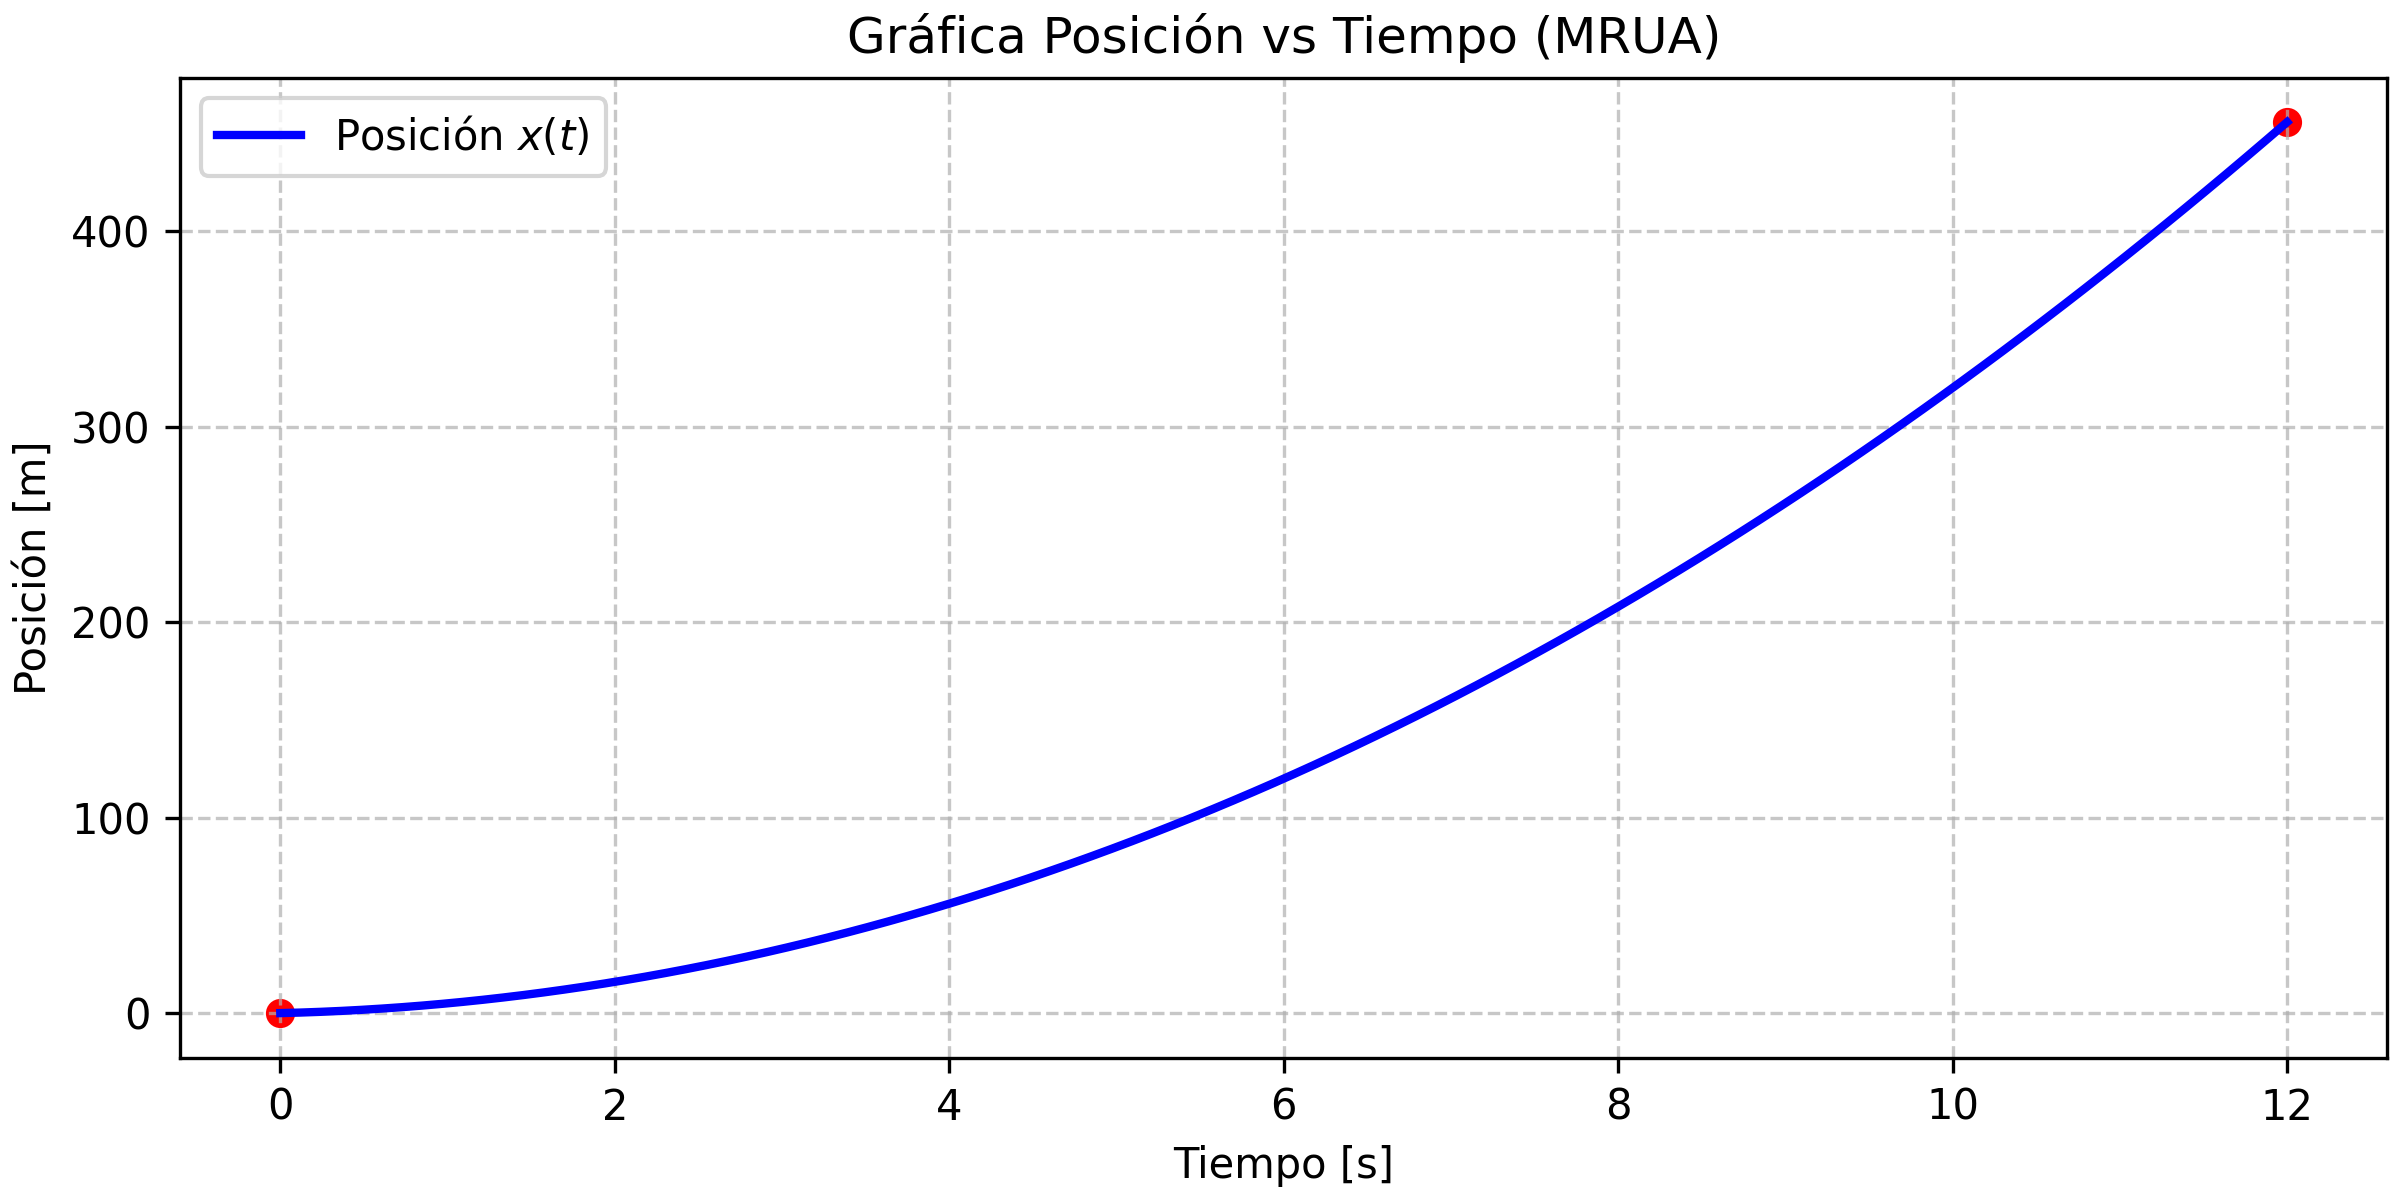
\includegraphics[width=0.8\textwidth]{grafico_2.png}
\end{center}

\vspace{0.5cm}
\textbf{Espacio para Resolución:}
\hrulefill
\vspace{1.5cm}
\hrulefill
\vspace{1.5cm}
\hrulefill
\vspace{1cm}


\newpage

% --- SECCIÓN DE RESPUESTAS ---
\section*{Clave de Respuestas}
A continuación se presentan los resultados numéricos para que puedas verificar tu trabajo:

\begin{enumerate}[label=\textbf{Ejercio \arabic*:}]
\item Posición Final: 204.00 m, Velocidad Final: 7.00 m/s

\item Posición Final: 456.00 m, Velocidad Final: 74.00 m/s

\end{enumerate}

\end{document}
